\documentclass{beamer}
\usepackage{listings}
\lstset{
%language=C,
frame=single, 
breaklines=true,
columns=fullflexible
}
\usepackage{subcaption}
\newtheorem{theorem}{Theorem}[section]
\newtheorem{problem}{Problem}
\newtheorem{proposition}{Proposition}[section]
\newtheorem{lemma}{Lemma}[section]
\newtheorem{corollary}[theorem]{Corollary}
\newtheorem{example}{Example}[section]
\newtheorem{definition}[problem]{Definition}

\newcommand{\BEQA}{\begin{eqnarray}}
\newcommand{\EEQA}{\end{eqnarray}}
\newcommand{\define}{\stackrel{\triangle}{=}}
\bibliographystyle{IEEEtran}
\raggedbottom
\setlength{\parindent}{0pt}
\providecommand{\mbf}{\mathbf}
\providecommand{\pr}[1]{\ensuremath{\Pr\left(#1\right)}}
\providecommand{\qfunc}[1]{\ensuremath{Q\left(#1\right)}}
\providecommand{\sbrak}[1]{\ensuremath{{}\left[#1\right]}}
\providecommand{\lsbrak}[1]{\ensuremath{{}\left[#1\right.}}
\providecommand{\rsbrak}[1]{\ensuremath{{}\left.#1\right]}}
\providecommand{\brak}[1]{\ensuremath{\left(#1\right)}}
\providecommand{\lbrak}[1]{\ensuremath{\left(#1\right.}}
\providecommand{\rbrak}[1]{\ensuremath{\left.#1\right)}}
\providecommand{\cbrak}[1]{\ensuremath{\left\{#1\right\}}}
\providecommand{\lcbrak}[1]{\ensuremath{\left\{#1\right.}}
\providecommand{\rcbrak}[1]{\ensuremath{\left.#1\right\}}}
\theoremstyle{remark}
\newtheorem{rem}{Remark}
\newcommand{\sgn}{\mathop{\mathrm{sgn}}}
\providecommand{\abs}[1]{\vert#1\vert}
\providecommand{\res}[1]{\Res\displaylimits_{#1}} 
\providecommand{\norm}[1]{\lVert#1\rVert}
%\providecommand{\norm}[1]{\lVert#1\rVert}
\providecommand{\mtx}[1]{\mathbf{#1}}
\providecommand{\mean}[1]{E[ #1 ]}
\providecommand{\fourier}{\overset{\mathcal{F}}{ \rightleftharpoons}}
%\providecommand{\hilbert}{\overset{\mathcal{H}}{ \rightleftharpoons}}
\providecommand{\system}{\overset{\mathcal{H}}{ \longleftrightarrow}}
	%\newcommand{\solution}[2]{\textbf{Solution:}{#1}}
\newcommand{\cosec}{\,\text{cosec}\,}
\renewcommand{\vec}[1]{\mathbf{#1}}
\providecommand{\dec}[2]{\ensuremath{\overset{#1}{\underset{#2}{\gtrless}}}}
\newcommand{\myvec}[1]{\ensuremath{\begin{pmatrix}#1\end{pmatrix}}}
\newcommand{\mydet}[1]{\ensuremath{\begin{vmatrix}#1\end{vmatrix}}}
\newcommand*{\permcomb}[4][0mu]{{{}^{#3}\mkern#1#2_{#4}}}
\newcommand*{\perm}[1][-3mu]{\permcomb[#1]{P}}
\newcommand*{\comb}[1][-1mu]{\permcomb[#1]{C}}
\usepackage[export]{adjustbox}
\usepackage[utf8]{inputenc}
\usepackage{amsmath}
\usetheme{Boadilla}
\usepackage{mathalfa}


\title{Construction : Q2.8}
\author{Tanay Yadav - AI20BTECH11026}
\date{\today}
\begin{document}
\begin{frame}
\titlepage
\end{frame}
\section{Question}
\begin{frame}
    \frametitle{Question}
    \begin{block}{Construction Q2.8}
        Can you construct a quadrilateral MIST where $MI = 3.5$, $IS = 6.5$, $\angle M = 100^{\circ}$, $\angle I = 105^{\circ}$, and $\angle S = 120^{\circ}$.
    \end{block}
\end{frame}
\begin{frame}
    \frametitle{Lemma 1}
    \begin{block}{}
    \begin{enumerate}
    \item[1.]Any Vector $\vec{X}$ can be expressed as:
    \begin{align}
        \vec{X} &= \vec{A} + x\vec{H}
    \end{align}
    where,
    \begin{enumerate}
        \item $\vec{A}$ is the tail of the vector $\vec{X}$,
        \item $x$ is the magnitude of the required vector $\vec{X}$,
        \item $\vec{H}$ is the unit vector in the direction of the vector $\vec{X}$.
    \end{enumerate}
    
    \item[2.]$\vec{H}$ is given as
    \begin{align}
        \vec{H} &= \myvec{\cos(\theta)\\\sin(\theta)}
    \end{align}
    where, $\theta$ is the angle made by the vector $\vec{X}$ with the positive x-axis.
    \end{enumerate}
    \end{block}
\end{frame}
\begin{frame}
    \frametitle{Lemma 1}
    \begin{block}{}
        Addition of two such vectors ($\vec{x}$, $\vec{y}$) can be written as:
    \begin{align}
        \vec{x} &= \vec{A} + x\vec{H}\\
        \vec{y} &= \vec{B} + y\vec{K}\\
        \therefore \vec{x} + \vec{y} &= \vec{A} + \vec{B} + x\vec{H} + y\vec{K}\\
       \therefore \vec{x} + \vec{y} &= \myvec{\vec{A} + \vec{B}} + \myvec{\vec{H} & \vec{K}}\myvec{x\\y}
    \end{align}
    \end{block}
\end{frame}
\begin{frame}
    \small
    \frametitle{Solution}
    \begin{block}{Given}
\begin{align}
    \norm{\vec{MI}} &= 3.5\\
    \norm{\vec{IS}} &= 6.5\\
    \angle{TMI} &= 100^{\circ}\\
    \angle{MIS} &= 105^{\circ}\\
    \angle{IST} &= 120^{\circ}
\end{align}
    \end{block}
    \begin{block}{If Quadrilateral MIST is possible}
        \begin{align}
    \therefore \angle{STM} &= 360 - 100 - 105 - 120\\
    \angle{STM} &= 35^{\circ}\\
    \text{Let, } \norm{\vec{ST}} &= x\\
    \norm{\vec{TM}} &= y
\end{align}\\
    \end{block}
\end{frame}
\begin{frame}
\small
    \frametitle{Solution}
    \begin{block}{}
    Considering $\vec{O} = \myvec{0\\0}$ to be the midpoint of $\vec{IS}$.
\begin{align}
    \therefore\norm{\vec{IO}} &= 3.25\\
    \norm{\vec{OS}} &= 3.25\\
\end{align}
The vectors are along the x-axis. Hence the coordinates are:
\begin{align}
    \therefore \vec{I} &= \myvec{-3.25\\0}\\
    \vec{S} &= \myvec{3.25\\0}
\end{align}
Using Lemma 1,
\begin{align}
    \because \angle MIS &= 105^{\circ}
    \end{align}
    \end{block}
\end{frame}
\begin{frame}
    \frametitle{Solution}
    \begin{block}{}
        \small
        \begin{align}
            \therefore \vec{M} &= \myvec{-3.25 + \norm{{\vec{MI}}}\cos({\angle{MIS}})\\0 + \norm{\vec{MI}}\sin({\angle{MIS}})}\\
            \therefore \vec{M} &= \myvec{-4.15\\3.38}
        \end{align}
        Now by Lemma 1,
        \begin{align}
            \vec{T} &= \vec{S} + x\myvec{\cos(180-\angle IST)\\\sin(180-\angle IST)}.
        \end{align}
        Now, the angle made by $\vec{MI}$ with negative x-axis is $180-105 = 75^{\circ}$. \\
        $\therefore$ The angle made by $\vec{TM}$ with x-axis: $ \alpha = (75-35) = 40^{\circ}$.
        Hence,
        \begin{align}
            \vec{T} &= \vec{M} + y\myvec{\cos(180 - \alpha)\\ \sin(180 - \alpha)}
        \end{align}
    \end{block}
\end{frame}
\begin{frame}
\small
    \frametitle{Solution}
    \begin{block}{}
        \small
        \begin{align}
            \therefore \vec{S} +     x\myvec{\cos(60)\\\sin(60)} &= \vec{M} + y\myvec{\cos(140)\\\sin(140)}\\
            \therefore \myvec{3.25\\0} + x\myvec{0.5\\0.86} &= \myvec{-4.15 \\ 3.38} + y\myvec{-0.76\\0.64}
        \end{align}
        Using Lemma 1,
        \begin{align}
            \myvec{0.5 & 0.76\\ 0.86 & -0.64}\myvec{x\\y} &= \myvec{-7.4\\3.38} \label{eq28}
        \end{align}
        Let
        \begin{align}
            \vec{A} &= \myvec{0.5 & 0.76\\ 0.86 & -0.64}\\
            \mydet{\vec{A}} &= -0.97
        \end{align}
        $\therefore \vec{A}^{-1}$ exists. 
    \end{block}
\end{frame}
\begin{frame}
    \frametitle{Solution}
    \begin{block}{}
        Calculating $\vec{A}^{-1}$ by adjoint method,
        \begin{align}
            \vec{A}^{-1} &= \dfrac{1}{\mydet{\vec{A}}}(adjoint(\vec{A}))\\
            \therefore \vec{A}^{-1} &= \myvec{0.66 & 0.78\\ 0.88 & -0.51}
        \end{align}
        Pre-multiplying $\vec{A}^{-1}$ to \eqref{eq28},
        \begin{align}
            \myvec{1 & 0\\0 & 1} \myvec{x\\y} &= \myvec{0.66 & 0.78\\ 0.88 & -0.51} \myvec{-7.4\\3.38}\\
            \therefore \myvec{x \\ y} &= \myvec{-2.24\\-8.23}\\
            \therefore x &= -2.24\\
            y &= -8.23
        \end{align}
    \end{block}
\end{frame}
\begin{frame}
    \frametitle{}
    \begin{block}{}
        But, $x$ and $y$ are magnitudes of $\vec{ST}$, $\vec{TM}$ and hence are always positive.\\
        Hence, a quadrilateral cannot be constructed using the given parameters.
        \\The adjacent python plot shows that this quadrilateral cannot be constructed.
        \begin{figure}
            \centering
            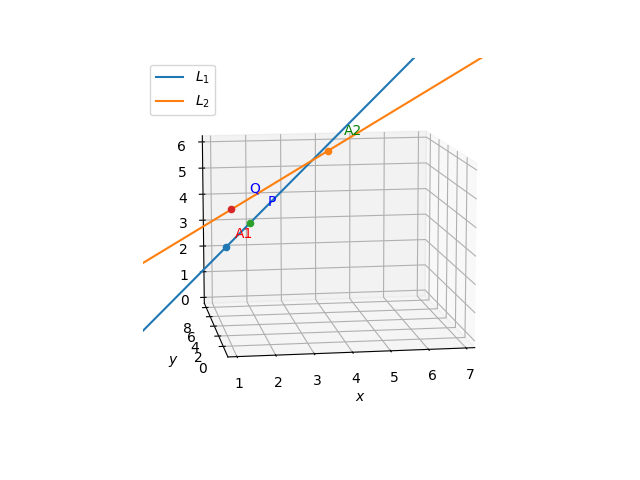
\includegraphics[scale = 0.4]{Figure_1.png}
        \caption{Plot for Quadrilateral MIST}
        \label{fig:my_label}
        \end{figure}
    \end{block}
\end{frame}
\end{document}